\documentclass[12pt, a4paper]{article}

\usepackage{tikz}
\usetikzlibrary{shapes.geometric}    % trapezium
\usetikzlibrary{arrows}              % arrow tips
\usepackage{amsmath, amsfonts}
\usepackage{bm}                      % boldsymbol
\usepackage{makecell}                % makecell
\usetikzlibrary{matrix,calc}
\usepackage{color}
\usepackage{xcolor}
\usepackage{multicol}
\definecolor{mygray}{HTML}{F0F0F0}
\definecolor{myred}{HTML}{CD594A} 
\definecolor{mygreen}{HTML}{829356} 
\definecolor{myblue}{HTML}{3C6478} 
\usepackage{mathtools}
\usetikzlibrary{decorations.pathreplacing}

\newcommand{\trans}{\text{T}}
\newcommand{\inv}{{-1}}
\newcommand{\eins}{\mathds{1}}
\DeclareMathOperator{\E}{\mathbb{E}}
\DeclareMathOperator{\I}{\mathbb{I}}
\newcommand{\tbf}[1]{\textbf{#1}}
\DeclareMathOperator{\tr}{tr}
\newcommand{\D}{\mathbf{D}}
\newcommand{\K}{\mathbf{K}}

\definecolor{mygray}{HTML}{F0F0F0}

\begin{document}

\begin{figure}[h!]
  \begin{minipage}{0.5\linewidth}
    \centering
    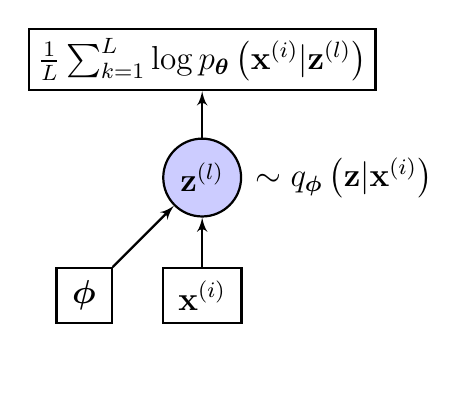
\begin{tikzpicture}[baseline=0, >=latex',thick] 
      % \node [rectangle, name=phi, minimum size=25pt] at (0,0) {\large{$\bm{\phi}$}};

      \node at (0,-0.8) {};
      \node (rect) at (0,0)
      [draw,thick,minimum width=0.7cm,minimum height=0.7cm, name=phi]
      {\large{$\bm{\phi}$}};      
      \node (rect) at (1.5,0)
      [draw,thick,minimum width=1cm,minimum height=0.7cm, name=x]
      {\large{$\tbf{x}^{(i)}$}};      

      \node [draw=black,name=z, circle, fill=blue!20, minimum size=25pt] at (1.5,1.5)
      {\large{$\tbf{z}^{(l)}$}};
      \node at (3.3, 1.5) {\large{$\sim q_{\bm{\phi}} \left( \tbf{z} | \tbf{x}^{(i)}\right)$}};

      \node (rect) at (1.5,3)
      [draw,thick,minimum width=1cm,minimum height=0.7cm, name=exp]
      {\large{$ \frac{1}{L}
        \sum_{k=1}^{L} \log p_{\bm{\theta}} \left( \tbf{x}^{(i)} | \tbf{z}^{(l)}\right)$}};      

      \draw [->] (phi) -- (z);
      \draw [->] (x) -- (z);
      \draw [->] (z) -- (exp);
      
    \end{tikzpicture}~\\
    \textbf{a) Original Objective} 
  \end{minipage}
  \begin{minipage}{0.5\linewidth}
    \centering
    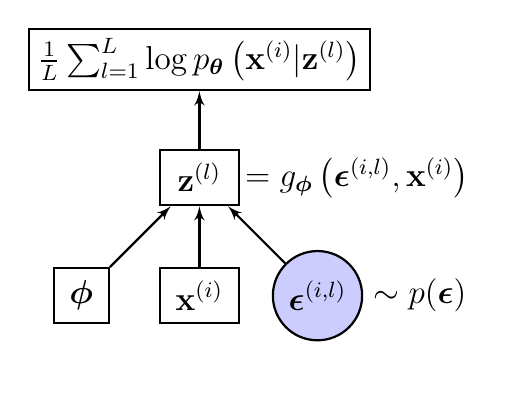
\begin{tikzpicture}[baseline=0, >=latex',thick] 
      \node at (0,-0.8) {};
      \node (rect) at (0,0)
      [draw,thick,minimum width=0.7cm,minimum height=0.7cm, name=phi]
      {\large{$\bm{\phi}$}};      
      \node (rect) at (1.5,0)
      [draw,thick,minimum width=1cm,minimum height=0.7cm, name=x]
      {\large{$\tbf{x}^{(i)}$}};      

      \node (rect) at (1.5,1.5)
      [draw,thick,minimum width=1cm,minimum height=0.7cm, name=z]
      {\large{$\tbf{z}^{(l)}$}};      

      \node [draw=black,name=epsilon, circle, fill=blue!20, minimum size=25pt] at (3,0)
      {\large{$\bm{\epsilon}^{(i,l)}$}};
      \node at (4.3, 0) {\large{$\sim p(\bm{\epsilon})$}};

      
      \node at (3.5, 1.5)
      {\large{$= g_{\bm{\phi}} \left( \bm{\epsilon}^{(i,l)} , \tbf{x}^{(i)}\right)$}};

      \node (rect) at (1.5,3)
      [draw,thick,minimum width=1cm,minimum height=0.7cm, name=exp]
      {\large{$\frac {1}{L}\sum_{l=1}^{L} \log p_{\bm{\theta}} \left( \tbf{x}^{(i)} | \tbf{z}^{(l)}\right)$}};      

      \draw [->] (phi) -- (z);
      \draw [->] (x) -- (z);
      \draw [->] (z) -- (exp);
      \draw [->] (epsilon) -- (z);
    \end{tikzpicture}~\\
    \textbf{b) Reparametrized Objective}
  \end{minipage}
\end{figure}

\end{document}
